\chapter{RSCP-iBGP系统的设计实现}
\label{cha:design}

\section{本章引言}
本文基于软件路由器Quagga\cite{quagga}的开源代码,实现了RSCP-iBGP内部域间路由协议系统。该系统主要分三部分:边界路由器、集中式的路由控制平台上运行的Route-Server、边界路由器与Route-Server之间的通信协议。本章首先介绍设计实现平台Quagga的概念以及其虚拟软件路由器上BGP的路由功能实现细节,之后介绍RSCP-iBGP系统的整体工作流程、模块设计以及复合式的路由算法,最后给出RSCP-iBGP系统的边界路由器、路由控制平台、通信接口三部分的具体实现。

\section{设计实现平台Quagga介绍}


\begin{figure}
  \centering
  % Requires \usepackage{graphicx}
  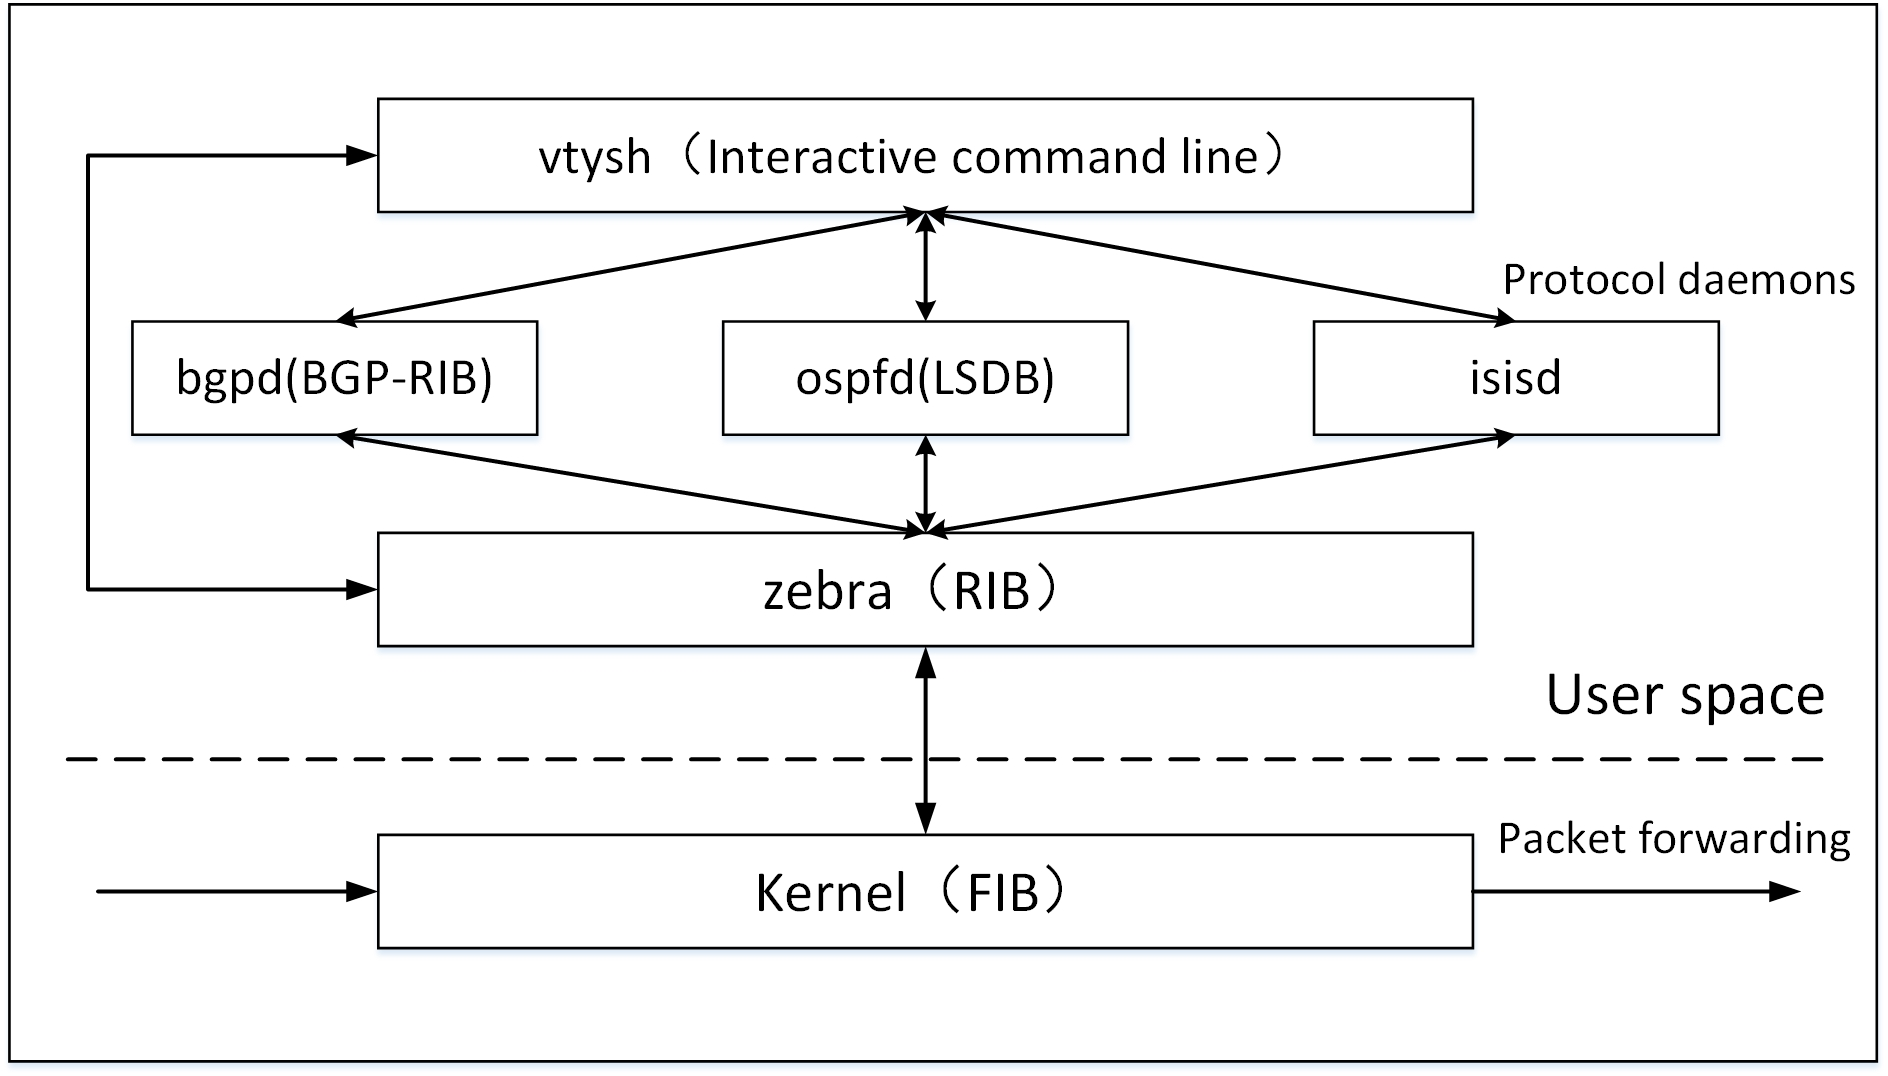
\includegraphics[width=0.75\textwidth]{quagga}
  \caption{Quagga系统结构图\cite{jakma2014quagga}}
  \label{fig:quagga}
\end{figure}


\subsection{基本概念及系统结构}
Quagga是一个比较成熟的虚拟路由器系统,该系统实现了多种网络协议,比如RIPv1、RIPv2、RIPng、OSPFv2、OSPFv3、BGPv4+、IS-IS等。Quagga中不同的网络协议需要运行不同的进程,属于多进程结构,协议之间相互独立,其本身的扩展性、维护性较强 \cite{quaggaThesis}。此外,Quagga中包含一个路由信息管理进程zebra,该进程和各种运行网络协议的进程通过ZServ协议进行交互,将运行网络协议进程产生的有效路由信息安装到内核\cite{jakma2014quagga}。每个协议进程均有自己的配置文件和终端接口,配置不同的网络需要在不同的网络进程内的配置文件中完成,非常麻烦。比如配置BGP网络时,需要在bgpd进程中的配置文件中完成;配置静态路由时,需要在zebra进程中的配置文件中完成。为此,Quagga存在vtysh进程来对Quagga中的其他进程进行配置。vtysh提供一个交互式的命令行接口来输入配置信息,其和其他进程通信通过一个简单的字符串传输协议。在vtysh进程中可以完成网络协议的配置、静态路由配置等对其余每一个进程的配置操作。Quagga的结构如图\ref{fig:quagga}。
\subsection{BGP协议的路由存储}

BGP协议中路由信息表有3种Adj-RIBs-In、Loc-RIB、Adj-RIBs-Out,Quagga中BGP协议的实现在bgpd进程中。bgpd进程中所有的数据结构均存储在bgp\_master结构体中,bgp\_master的成员变量中存在一个链表,包含了所有的bgp实例。每个bgp实例中存储了该BGP session的配置文件、一个链表包含所有的peer实例、静态路由表、路由表(Loc-RIB,结构体为bgp\_table)等信息。


\begin{figure}
  \centering
  % Requires \usepackage{graphicx}
  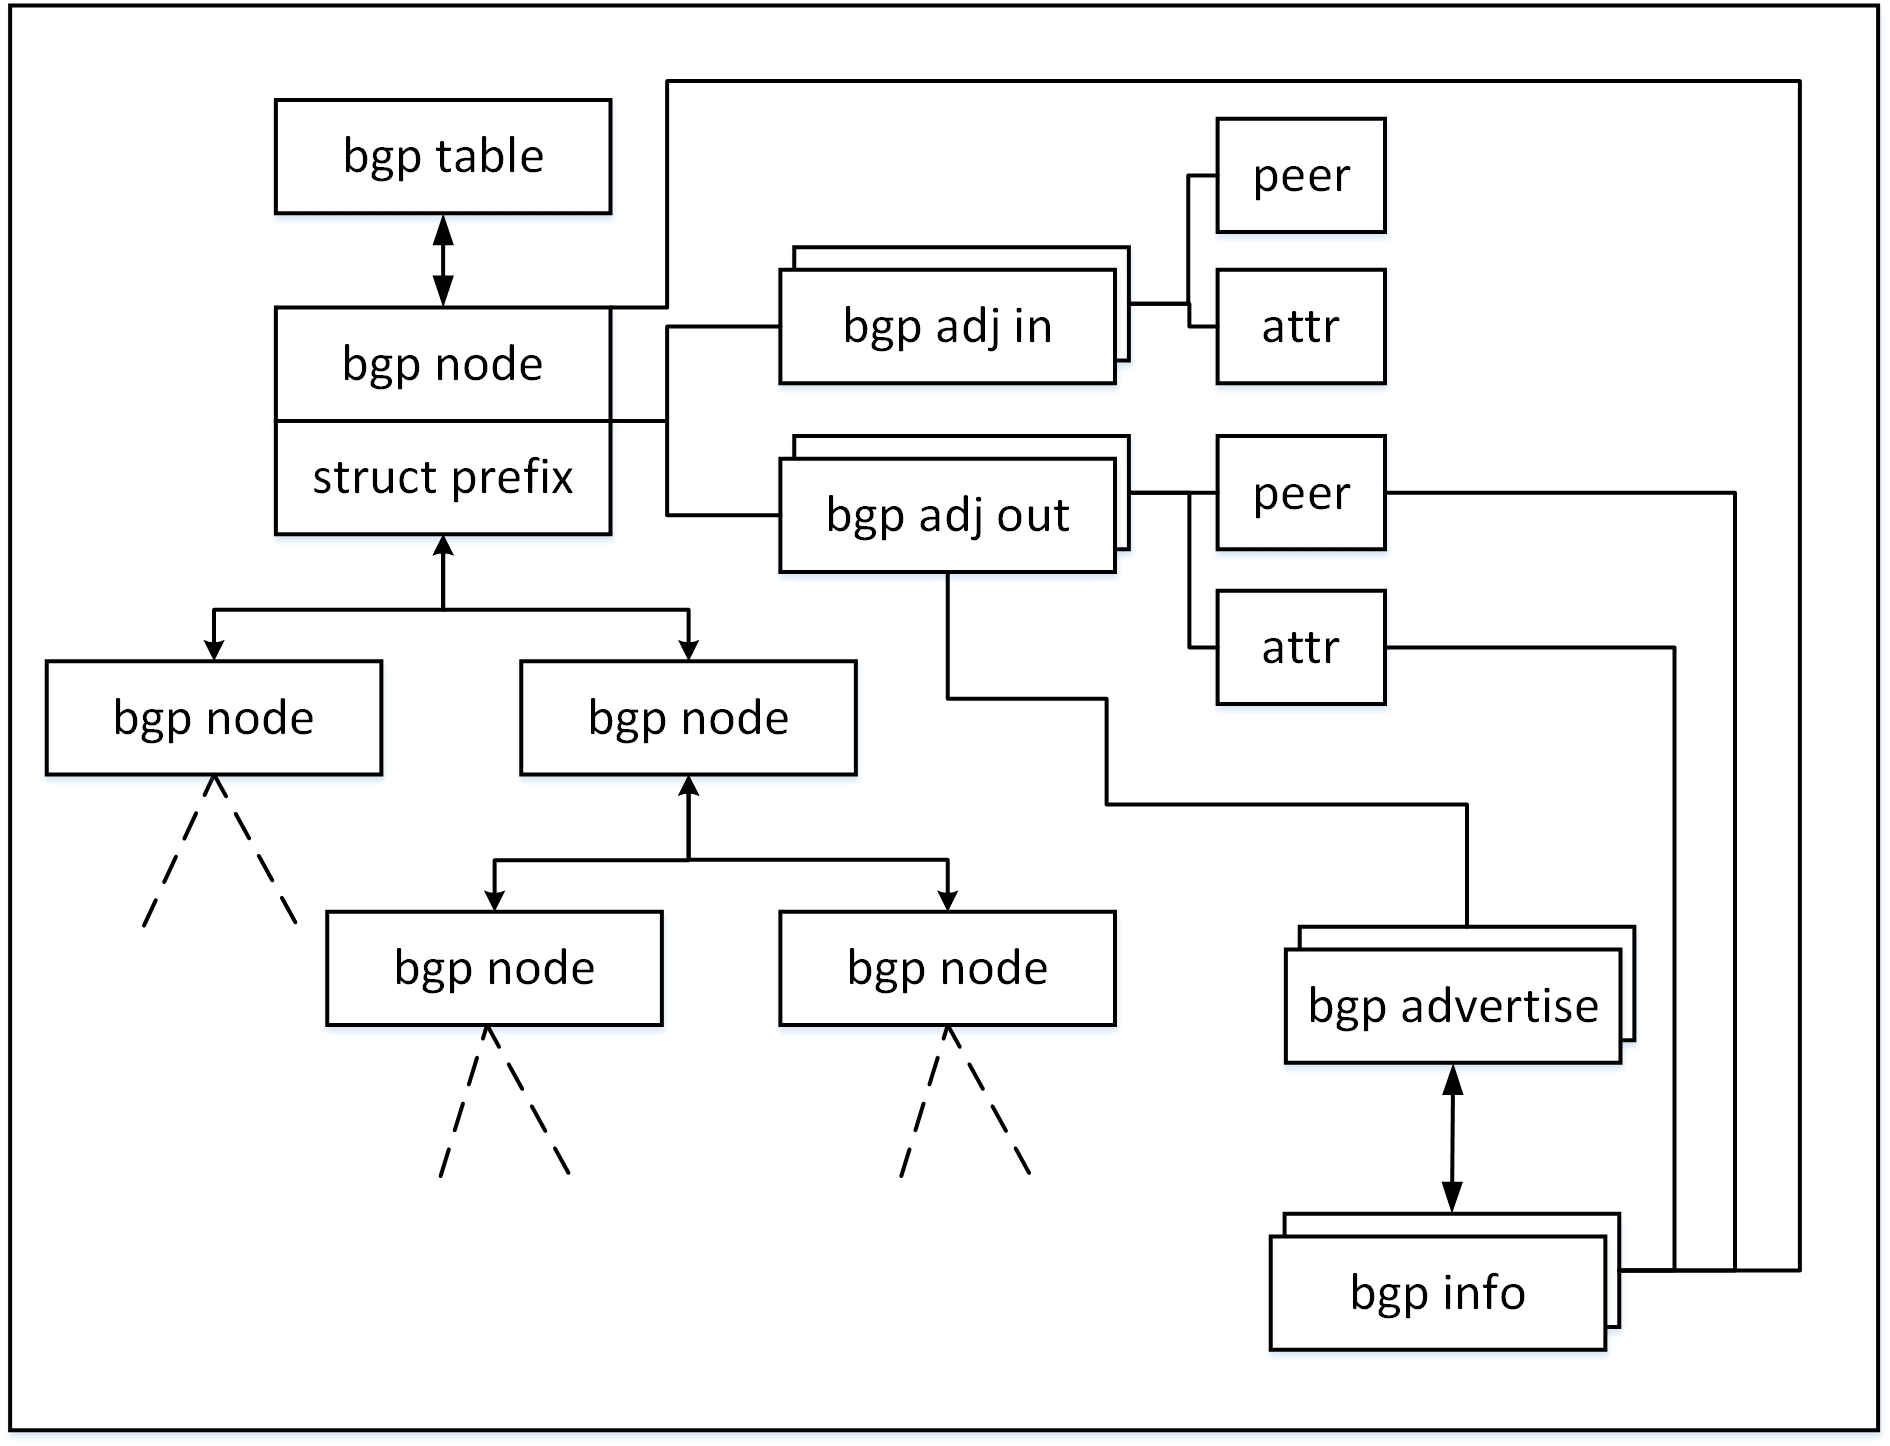
\includegraphics[width=0.75\textwidth]{storage}
  \caption{Quagga-bgpd:BGP路由表概括图\cite{jakma2014quagga}}
  \label{fig:storage}
\end{figure}

Quagga中路由表的存储使用radix二叉树\cite{quaggaThesis}存储结构,radix树是以二进制表示的键值作为树的节点,每个节点通过比较比特位来进行查找,radix二叉搜索树适合处理非常长的,可变长度的键值。每张Loc-RIB表存储在bgp\_table的结构体中,bgp\_table结构体有一个成员变量为bgp\_node类的结构体指针,该结构体指针是该Loc-RIB表radix树结构的根节点,所有路由表项的查找、删除等操作都从该根节点开始。bgp\_node结构体的实例代表的是某前缀所有的路由信息(每一条路由信息用bgp\_info结构体对应的实例表示),bgp\_node结构体中也存在指向bgp\_adj\_in和bgp\_adj\_out的指针。路由信息在bgp\_adj\_in和bgp\_adj\_out中的主要体现是通过他们的成员变量peer和attr。当BGP的某个邻居与之断开连接,则可以通过peer找到对应的prefix,清除bgp\_adj\_in且更新Loc-RIB。

当运行Quagga的虚拟路由器收到路有更新时,如果开启了Adj-RIBs-In存储设置,则会先根据前缀找到对应的bgp\_node,之后根据bgp\_node找到对应的adj\_rib\_in,对其进行更新。

针对某条路由信息bgp\_info向外进行路由宣告时,如果开启了Adj-RIBs-Out存储设置,则会先根据bgp\_info结构体中bgp\_node的指针,找到对应的bgp\_node,之后根据bgp\_node找到对应的adj\_rib\_out,对其进行更新。

综合以上的文字解释,Quagga中实现BGP三张表的存储结构如图\ref{fig:storage}。
\subsection{路由更新流程}

路由更新过程是虚拟路由器进行路由处理流程的主要部分,对应到Quagga中bgpd进程实现,路由更新的步骤如下:
\begin{itemize}
  \item 运行Quagga的虚拟路由器先通过bgp\_establish()函数与对等体peer建立连接;
  \item 运行Quagga的虚拟路由器通过bgp\_read()接收来自对等体的消息;
  \item 当收到BGP消息,通过检查头部的报文格式分析报文类型,如果是UPDATE报文,执行路由更新处理函数bgp\_update\_receive(),进行UPDATE报文解析bgp\_nlri\_parse();
  \item 报文解析结束后,执行bgp\_update()、bgp\_update\_main()等函数进入路由更新消息的处理;
  \item 路由更新消息处理的过程中:如果需要存储Adj-RIBs-In表,进入bgp\_adj\_in\_set()函数存储未经过滤的路由信息;之后执行入站过滤bgp\_input\_filter()、入站更新bgp\_input\_modifier();如果更新路由没有被过滤掉,则将更新路由其通过info\_make()函数生成bgp\_info信息;通过bgp\_info\_add()函数将bgp\_info结构体的信息加入Loc\_RIB表中,然后将其通过bgp\_process()函数将该bgp\_info路由信息的处理流程加入bgp\_process\_queue队列,该队列使用先进先出的策略;
  \item 当轮到该路由信息bgp\_info处理程序时,进入bgp\_process\_main()函数,执行最优路由计算bgp\_best\_selection();
  \item 如果该前缀对应的最优路由发生改变,则执行bgp\_process\_announce\_selected()函数,在该函数中有出站过滤更新bgp\_announce\_check()和Adj-RIBs-Out更新bgp\_adj\_out\_set();
  \item 最终通过bgp\_zebra\_announce()函数将BGP路由更新到RIB表中,以此影响FIB表。
\end{itemize}

\subsection{路由算法}

Quagga的bgpd进程中路由算法主要是在bgp\_best\_selection()函数中实现的。针对前缀Prefix,在bgp\_table中找到该前缀对应的所有路由信息bgp\_node。路由信息的存储使用链表的数据结构,最新的路由会插在表头,所以bgp\_node存储的同一前缀的路由信息是按照更新时间由近及远进行存储。将该前缀对应的路由信息由近及远两两通过bgp\_info\_cmp()进行比较,得到前缀的最优路由。两两比较的路由算法见章节\ref{subsec:calculation}。


\section{系统详细设计}
模块设计图总体、项目的模块设计

\subsection{系统的工作流程}

\subsection{系统的模块设计}

\subsection{复合式路由算法}


\section{系统实现}

\subsection{边界路由器}
路由宣告
\subsection{路由控制平台}
\subsubsection{路由存储}
\subsubsection{路由计算}
\subsection{通信接口}
BGP协议
\section{本章小结}
本章对SRCP-iBGP系统的实现平台Quagga进行了详细的介绍,了解虚拟路由器的BGP路由实现之后,更容易理解本文提出的SRCP-iBGP系统的设计与实现。
